%
% assembly.tex
%
% Copyright (C) 2021 by Universidade Federal de Santa Catarina.
%
% OBDH 2.0 Documentation
%
% This work is licensed under the Creative Commons Attribution-ShareAlike 4.0
% International License. To view a copy of this license,
% visit http://creativecommons.org/licenses/by-sa/4.0/.
%

%
% \brief Assembly instructions chapter.
%
% \author Gabriel Mariano Marcelino <gabriel.mm8@gmail.com>
%
% \institution Universidade Federal de Santa Catarina (UFSC)
%
% \version 0.7.0
%
% \date 2020/05/12
%

\chapter{Board Assembly} \label{ch:assembly}

The OBDH2 has some DNP components to provide flashing, debugging, testing or providing extra interfaces if needed. These components may not be necessary for the flight model of the board. The draftsman document can be viewed for more detailed information regarding their location and board dimensions \cite{obdh2-draftsman}.

\section{Development Model}

\subsection{Debug and programming connectors}

The P2 and P6 connectors are used for flashing and debugging the OBDH2 board. \hyperref[sec:programer-and-debug]{See again chapter 3 (Hardware) and subsection 3.2.3 (Programmer and Debug) for more information}.

\subsection{Status leds}

As already exposed before in the document OBDH2 has status leds to be used during development and test phases. \hyperref[sec:status-leds]{See again chapter 2 (System Overview) and the subsection 2.3.1 (Status Leds) for more information}.

\subsection{Analog circuits}

TBD

\section{Flight Model}

TBD

\section{Custom Configuration}

On the PC104 connector of OBDH2 there are some jumper resistors to enable extra I2C, SPI and GPIOs interfaces if desired. Note that the I2C0, I2C1 and SPI channels should not be used with shared devices. The corresponding table and location on the pcb of these components are showed below. 

\begin{table}[!h]
    \centering
    \begin{tabular}{cllll}
        \toprule[1.5pt]
        \textbf{Label} & \textbf{Interface} \\
        \midrule
        J\_PC1            & I2C0\_SDA \\
        J\_PC2            & I2C0\_SCL \\
        J\_PC3            & I2C1\_SDA \\
        J\_PC4            & I2C1\_SCL \\
        J\_PC5            & SPI\_MOSI \\
        J\_PC6            & SPI\_MISO \\
        J\_PC7            & SPI\_CLK \\
        J\_PC8            & GPI0 \\
        J\_PC9            & GPIO1 \\
        J\_PC10           & GPIO2 \\
        J\_PC11           & GPIO3 \\
        \bottomrule[1.5pt]
    \end{tabular}
    \caption{Additional PC104 inferfaces.}
    \label{tab:additional-pc104-inferfaces}
\end{table}

\begin{figure}[!ht]
    \begin{center}
         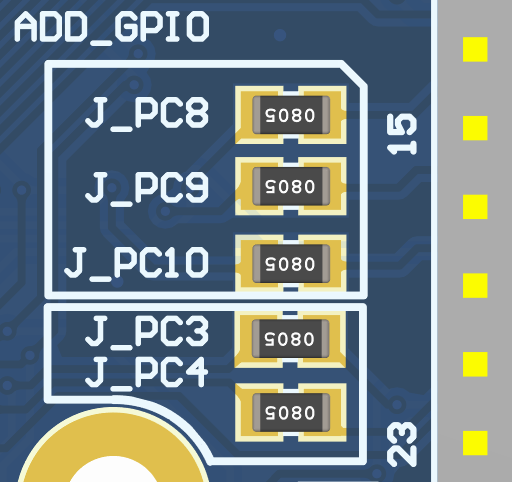
\includegraphics[width=55mm]{figures/add_gpio_i2c1_jumpers.png}
        \caption{Additional GPIOs and I2C channel 1.}
        \label{fig:add_gpio_i2c1_jumpers}
        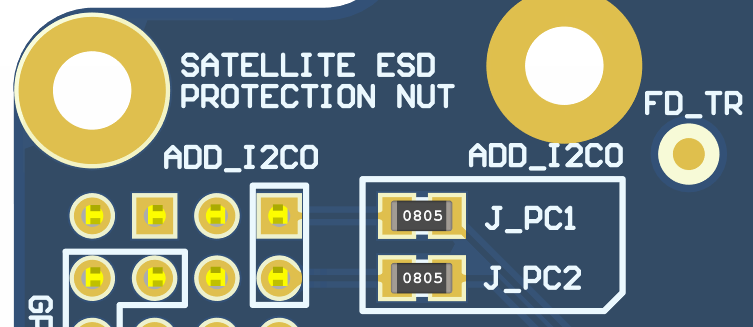
\includegraphics[width=90mm]{figures/add_i2c0_jumpers.png}
        \caption{Additional I2C channel 0.}
        \label{fig:add_i2c0_jumpers}
        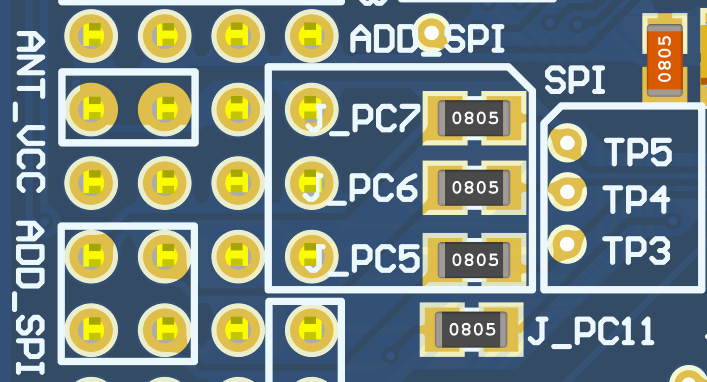
\includegraphics[width=80mm]{figures/add_spi_1gpio_jumpers.png}
        \caption{Additional GPIO and SPI channel.}
        \label{fig:add_spi_1gpio_jumpers}
    \end{center}
\end{figure}
